\documentclass[10pt]{article}
\setlength{\oddsidemargin}{0.25 in}
\setlength{\evensidemargin}{-0.25 in}
\setlength{\topmargin}{-0.6 in}
\setlength{\textwidth}{6.5 in}
\setlength{\textheight}{8.5 in}
\setlength{\headsep}{0.75 in}
\setlength{\parindent}{0 in}
\setlength{\parskip}{0.1 in}

\usepackage{graphicx}
\usepackage{url}

\usepackage{float}
\usepackage{hyperref}

%
% The following commands sets up the lecnum (lecture number)
% counter and make various numbering schemes work relative
% to the lecture number.
%
\newcounter{lecnum}
\renewcommand{\thepage}{\thelecnum-\arabic{page}}
%\renewcommand{\thesection}{\thelecnum.\arabic{section}}
\setcounter{section}{6}
\renewcommand{\theequation}{\thelecnum.\arabic{equation}}
%\renewcommand{\thefigure}{\thelecnum.\arabic{figure}}
\renewcommand{\thetable}{\thelecnum.\arabic{table}}
\newcommand{\dnl}{\mbox{}\par}

%
% The following macro is used to generate the header.
%
\newcommand{\lecture}[4]{
  \pagestyle{myheadings}
  \thispagestyle{plain}
  \newpage
  \setcounter{lecnum}{#1}
  \setcounter{page}{1}
  \noindent
  \begin{center}
  \framebox{
     \vbox{\vspace{2mm}
   \hbox to 6.28in { {\bf CMPSCI~630~~~Systems
                       \hfill Spring 2023} }
      \vspace{4mm}
      \hbox to 6.28in { {\Large \hfill Lecture #1  \hfill} }
%       \hbox to 6.28in { {\Large \hfill Lecture #1: #2  \hfill} }
      \vspace{2mm}
      \hbox to 6.28in { {\it Lecturer: #3 \hfill Scribe: #4} }
     \vspace{2mm}}
  }
  \end{center}
  \markboth{Lecture #1: #2}{Lecture #1: #2}
  \vspace*{4mm}
}

%
% Convention for citations is authors' initials followed by the year.
% For example, to cite a paper by Leighton and Maggs you would type
% \cite{LM89}, and to cite a paper by Strassen you would type \cite{S69}.
% (To avoid bibliography problems, for now we redefine the \cite command.)
%
\renewcommand{\cite}[1]{[#1]}

% \input{epsf}

%Use this command for a figure; it puts a figure in wherever you want it.
%usage: \fig{NUMBER}{FIGURE-SIZE}{CAPTION}{FILENAME}
%\newcommand{\fig}[4]{
%           \vspace{0.2 in}
%           \setlength{\epsfxsize}{#2}
%           \centerline{\epsfbox{#4}}
%           \begin{center}
%           Figure \thelecnum.#1:~#3
%           \end{center}
%   }

% Use these for theorems, lemmas, proofs, etc.
\newtheorem{theorem}{Theorem}[lecnum]
\newtheorem{lemma}[theorem]{Lemma}
\newtheorem{proposition}[theorem]{Proposition}
\newtheorem{claim}[theorem]{Claim}
\newtheorem{corollary}[theorem]{Corollary}
\newtheorem{definition}[theorem]{Definition}
\newenvironment{proof}{{\bf Proof:}}{\hfill\rule{2mm}{2mm}}

% Some useful equation alignment commands, borrowed from TeX
\makeatletter
\def\eqalign#1{\,\vcenter{\openup\jot\m@th
 \ialign{\strut\hfil$\displaystyle{##}$&$\displaystyle{{}##}$\hfil
     \crcr#1\crcr}}\,}
\def\eqalignno#1{\displ@y \tabskip\@centering
 \halign to\displaywidth{\hfil$\displaystyle{##}$\tabskip\z@skip
   &$\displaystyle{{}##}$\hfil\tabskip\@centering
   &\llap{$##$}\tabskip\z@skip\crcr
   #1\crcr}}
\def\leqalignno#1{\displ@y \tabskip\@centering
 \halign to\displaywidth{\hfil$\displaystyle{##}$\tabskip\z@skip
   &$\displaystyle{{}##}$\hfil\tabskip\@centering
   &\kern-\displaywidth\rlap{$##$}\tabskip\displaywidth\crcr
   #1\crcr}}
\makeatother

% **** IF YOU WANT TO DEFINE ADDITIONAL MACROS FOR YOURSELF, PUT THEM HERE:



% Some general latex examples and examples making use of the
% macros follow.

\begin{document}

%\lecture{**LECTURE-NUMBER**}{**DATE**}{**LECTURER**}{**SCRIBE**}
\lecture{7}{March 7}{Emery Berger}{Victor L.}

\section{Hardware/Software Interface}
In this lecture we discussed the evolution of ISA and why they continued to grow for so many yeras and also covered CISC and RISC, with some examples from Intel. 

\subsection{Instruction Set Architectures (ISA)}
Assembly language is a very high level language with respect to the machine code and hardware. For example: \texttt{add \$1 \$2 \$3} is the MIPS x86 representation of the add command. When we get to hardware, things get a lot more complicated. In figure \ref{fig:1}, we see the circuit diagram of a 1-bit adder, the hardware that actually executes the instruction. To be able to operate on larger numbers (more than 1-bit), we need many of these in parallel, with the carry-out wire $C_{out}$ tied to the next adders carry-in wire $C_{in}$.  
\begin{figure}[H]
\centering
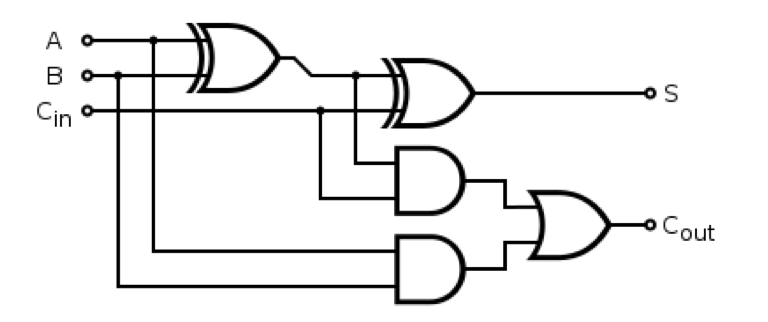
\includegraphics[width=10cm]{full_adder.png}
\caption{Full Adder \cite{\href{http://www.cs.cmu.edu/~tcortina/15110m14/Unit08PtB.pdf}{C4}}}
\label{fig:1}
\end{figure}
There are various levels from abstraction, from high level programming languages (e.g. C++), which are compiled down to assembly, then assembled into machine code. Operating at a lower level gives us more control over the computer and allows us to do optimizations not possible at higher levels.\\
\newline
The minimum for an assembly language to be Turing complete is simple; any assembly language capable of: \texttt{read, store, if \$1==0 -> goto \$2} are Turing complete. Being Turing complete however is not an indicator of a good assembly language, as this example would only allow us to perform operations on data 1-bit at a time. There are some trade-offs that must be considered when designing an ISA such as the abstraction level, the number of instructions, and the complexity of decoding.\\
\newline
Many companies, especially Intel, started added an abundance of instructions into the ISA hoping for better performance, support of more programming languages, and easier compilation of programs. In the '70s and '80s, many specialized CPUs were created. These CPUs would be entirely single purpose (like embedded systems) and would have ISAs that only supported certain applications, like database operations, running JVM, and even one that only ran LISP instructions (called the \href{https://en.wikipedia.org/wiki/Lisp_machine}{LISP-machine}). This belief that dedicated hardware circuits would always outperform software is true for the most part. Take for example implementing the square-root function. The \href{https://en.wikipedia.org/wiki/Newton\%27s_method}{Newton-Raphson} algorithm takes $\log n$ operations as it makes a guess, averages the guess with the quotient and "guesses" again, performing a sort of binary search. This is a lot of instructions as this will run recursively. In hardware, much of the overhead of executing an instruction like this could be removed as there's no fetch, decode, or execute cycles; you would just pass the circuit the operand and get the answer. However, dedicated circuits take up space on the silicon. This was, however, not a big concern at the time as Moore's law still held.\\
\newline
With high level programming languages, there are often a lot of small things that are abstracted away to make programming easier. In C++, if we have for example a class variable (e.g. \texttt{vector<int>}) and call a function of the class (\texttt{vector.push\_back()}), the address of the instructions to execute this function are stored in a virtual dispatch table (\href{https://pabloariasal.github.io/2017/06/10/understanding-virtual-tables/}{vtable}). There is a table for every class so we need to check the class "tag" of the variable to find it's vtable. So for every class function call, there is quite a bit of extra work that must be done.\\
\subsection{Complex Instruction Set Computer (CISC)}
A lot of instructions added to ISAs are inspired by the actual code found in programs. Intel added an instruction, \texttt{REP}, to work with \texttt{MOV}. Together, these instructions would allow you to move characters of a string (or any other data) from one location to another. A lot of these instructions that were added required the use of special hardware, and so were extremely complex and often of various lengths. This required that the processor have a more complex decoder to decipher what each instruction was, and this stage could take a long time as the decode would have to on the fly figure out the length of the instruction as well. With the introduction of so many instructions were new security risks. Many of these instructions were unchecked and were just blindly executed by the CPU. An attacker could for example perform code injection through a buffer overflow attack to a region of memory that stores frequently used code (e.g. destructor), and know their code would eventually be run.\\
\newline
Having a complex decoder allowed more specialized instructions to be supported by the ISA, but it came at the cost of increased latency. The second stage of most processor pipelines is the decode stage which usually only takes one cycle. However, now that the instructions are more complicated, either cycle time needs to increase, decreasing the throughput, or split the decode stage into multiple stages lengthening the pipeline.\\
\newline
Having such a large multitude of instructions also caused other problems. There were often instructions that were very similar, and differed ever so slightly that it was extremely hard to differentiate. The problem of instruction selection for compilers became harder as it there were too many options and it wasn't immediately apparent how they differed. As a compiler writer, it is hard to determine when to use each instruction, and even harder to write a compiler that can make the differentiation.\\
\subsection{Reduced Instruction Set Computer}
RISC's ISA offers a more limited instruction set as well as uniform instruction size. This comes with many benefits such as being easier to write compilers and optimize code. Having uniform instruction sizes allows for pre-fetching of instructions as well as easier and faster decoding. Caching of instructions is also easier as we can store a set number of instructions in one cache line. All this makes it really easy to pipeline a RISC processor as instruction fetch and decode are so straightforward. The simplicity of RISC allows processors to have lower depth circuits, leading to better energy efficiency, and less heat produced. As a result, nearly every mobile processor is based on RISC.
\newline
John L Hennessy and David A Patterson, the author of \textit{The Case for the Reduced Instruction Set Computer} (and later both authors of \textit{Computer Architecture: A Quantitative Approach}) banked on RISC being the future of computer architecture. Hennessy and Patterson both lead a group of companies (MIPS Computer and Sun Microsystems respectively) to work on the development of a RISC processor. Sun Microsystems today is a part of Oracle.\\
\subsection{Intel Chips}
It is doubtful that today, there are actually any "pure" CISC architectures left (n.b. CISC and RISC have no formal definition). Intel's chips claim to be based on a CISC architecture, however there is a RISC core on chip. They translate x86 instructions to microinstructions (a lower-level instruction set) before execution by its RISC-like core. There are however still non-RISC instructions as part of the ISA (Since Intel almost never removes an instruction once it has been added) and other processing units to execute the non-RISC instructions. These other processing units are marketed to us as accelerators (e.g. NPU). Other units now included with Intel chips include a true RNG (based on quantum states) and support for cryptocurrency operations.\\
\newline
The Intel 8088 ISA had hardware support for integers and performed floating point operations in software; floating point instructions were prefixed with an 'F'. IBM designed a computer with two CPU slots, one for the Intel 8088 and the other for the Intel 8087. The 8087 was just a floating point unit and any floating point instruction would be sent from the 8088 to the 8087, which would then return the result back to the 8088. Eventually, these became unified into a single chip.\\
\newline
There are often instructions that we want to be performed on hardware as it is significantly faster. Field programmable gate arrays (FPGA) (exactly what it sounds like) are a good solution to this problem. It can be thought of as Lego blocks (logic-gates) that we put together at run-time to form any circuit we need. As a result, they are now found in many computers such as Microsoft Azure servers. An example of the speedup that can be realized from an FPGA is with AES encryption. The Xilinx Zynq 7000 processor has a 667MHz clock and a 17,000 LUT FPGA. On the processor, it is able to perform 16-bit encryption at 3Mbps maximum. Implementing an AES core on the FPGA, we are able to get 50Mbps, a nearly 20x speedup.\\
\newline
Intel computers for many years were akin to Porsches. They were designed with only performance in mind without regard for power consumption and they were very expensive. ARM, a company that designs RISC based processors and licenses them out, started designing chips but they weren't fighting Intel for marketshare. ARMs primary sector was embedded systems as they were often resource constrained, so they were incapable of supporting an Intel processor. Fast forward a few years and Intel's chips are now as fast as they can get and mobile computing platforms (cellphones) are now the most popular computing platform. Intel has none of this marketshare as there is not a phone in the world capable of powering the chip and dissipating the heat given off. ARM chips are relatively low power and don't have a heating issue so they end up taking over the market. Intel tries to develop an energy efficient chip (the first being the Atom); the Atom turned out to not be so energy efficient and it was extremely slow. 

\end{document}
